%%%%%%%%%%%%%%%%%%%%%%%%%
\section{State of the Art} \label{stateOfTheArt}
%%%%%%%%%%%%%%%%%%%%%%%%%
City visualization is a subject undergoing intense study, therefore it is easy to find new projects about it everyday, on the Internet. Still, the uniqueness of \applicationName\ resides on the fact that it provides not only a visualization of a city but, above all, it gives the user the possibility to interact with the city itself through a simple system of visual queries.\\

Before getting into the details with \applicationName, we will clarify the current state of city visualization and, since the projects about this topic are so various and so many, in this Chapter, we will present the ones that relate most with the final outcome of this Bachelor Project.\\

At first, we will present some 3D--city--model based on OpenStreetMap data, as {\bf OSMBuildings}, {\bf F4 Map} and {\bf ViziCities}. Then, we will introduce the {\bf Cesium framework}, since it has been used used as a basis for \applicationName. At the end, we will analyze the work done by the {\bf Swiss Geospatial Portal} (still using Cesium), in order to compare it with the application described in this report. 
\subsection{OpenStreetMap--Based Frameworks}
OpenStreetMap\footnote{OpenStreetMap: phttp://www.openstreetmap.org/} is a project that creates and distributes free geographic data for the world. During the last decade, the third dimension has become a growing topic at OSM, so it is now possible to add detailed buildings and a lot of minor objects. Here, some of the frameworks that use this data, will be analyzed.
\subsubsection{OSMBuildings}
OSMBuildings\footnote{OSMBuildings: https://osmbuildings.org/} is an engine for displaying 3D buildings on a web map. It uses information on buildings provided by OpenStreetMap and it renders them on a map layer.\\Altough in some cases, buildings are very detailed (e.g., in big cities like New York or Berlin), it does only provide a visualization without any kind of interaction.
\begin{figure} [H]
\centering
\includegraphics[width=0.8\textwidth]{chapter2/images/OSM_Building}
\caption{A visualization of New York city using OSMBuildings}
\label{fig:OSM_Building}
\end{figure}

\subsubsection{F4 Map}
The F4 Map\footnote{F4 Map: http://demo.f4map.com/} is an OSM-based 3D map using the WebGL technology. Also this map, uses Open Street Map's buildings but also adds some non--OSM--provided features like trees, cranes and other data.\\
 Some 3D models are used (not based on buildings data in OpenStreetMap) for some specific buildings (e.g. the Eiffel Tower in the example below).
\begin{figure}[H]
\centering
\includegraphics[width=0.8\textwidth]{chapter2/images/F4-Map}
\caption{A visualization of Paris using F4 Map}
\label{fig:F4-Map}
\end{figure}
Unfortunately, the F4 group does not provide any kind of documentation and this project is not open source.
\subsubsection{ViziCities}
The third and last map that uses OSM information about buildings is ViziCities\footnote{ViziCities: https://github.com/UDST/vizicities} , a framework for 3D geospatial visualization in the browser. Its code is available on GitHub since it is an OpenSource project but they are still at version 0.3 of the application.\\It lets the developer to add some useful information to the map like routes and GeoJSON (i.e., a format for encoding a variety of geographic data structures) but is still very limited and not very prone to interactivity.
\begin{figure}[H]
\centering
\includegraphics[width=0.8\textwidth]{chapter2/images/vizicities-Map}
\caption{A visualization of New York city using ViziCities}
\label{fig:vizicities-Map}
\end{figure}

\subsection{Cesium}
\begin{figure} [h]
\centering
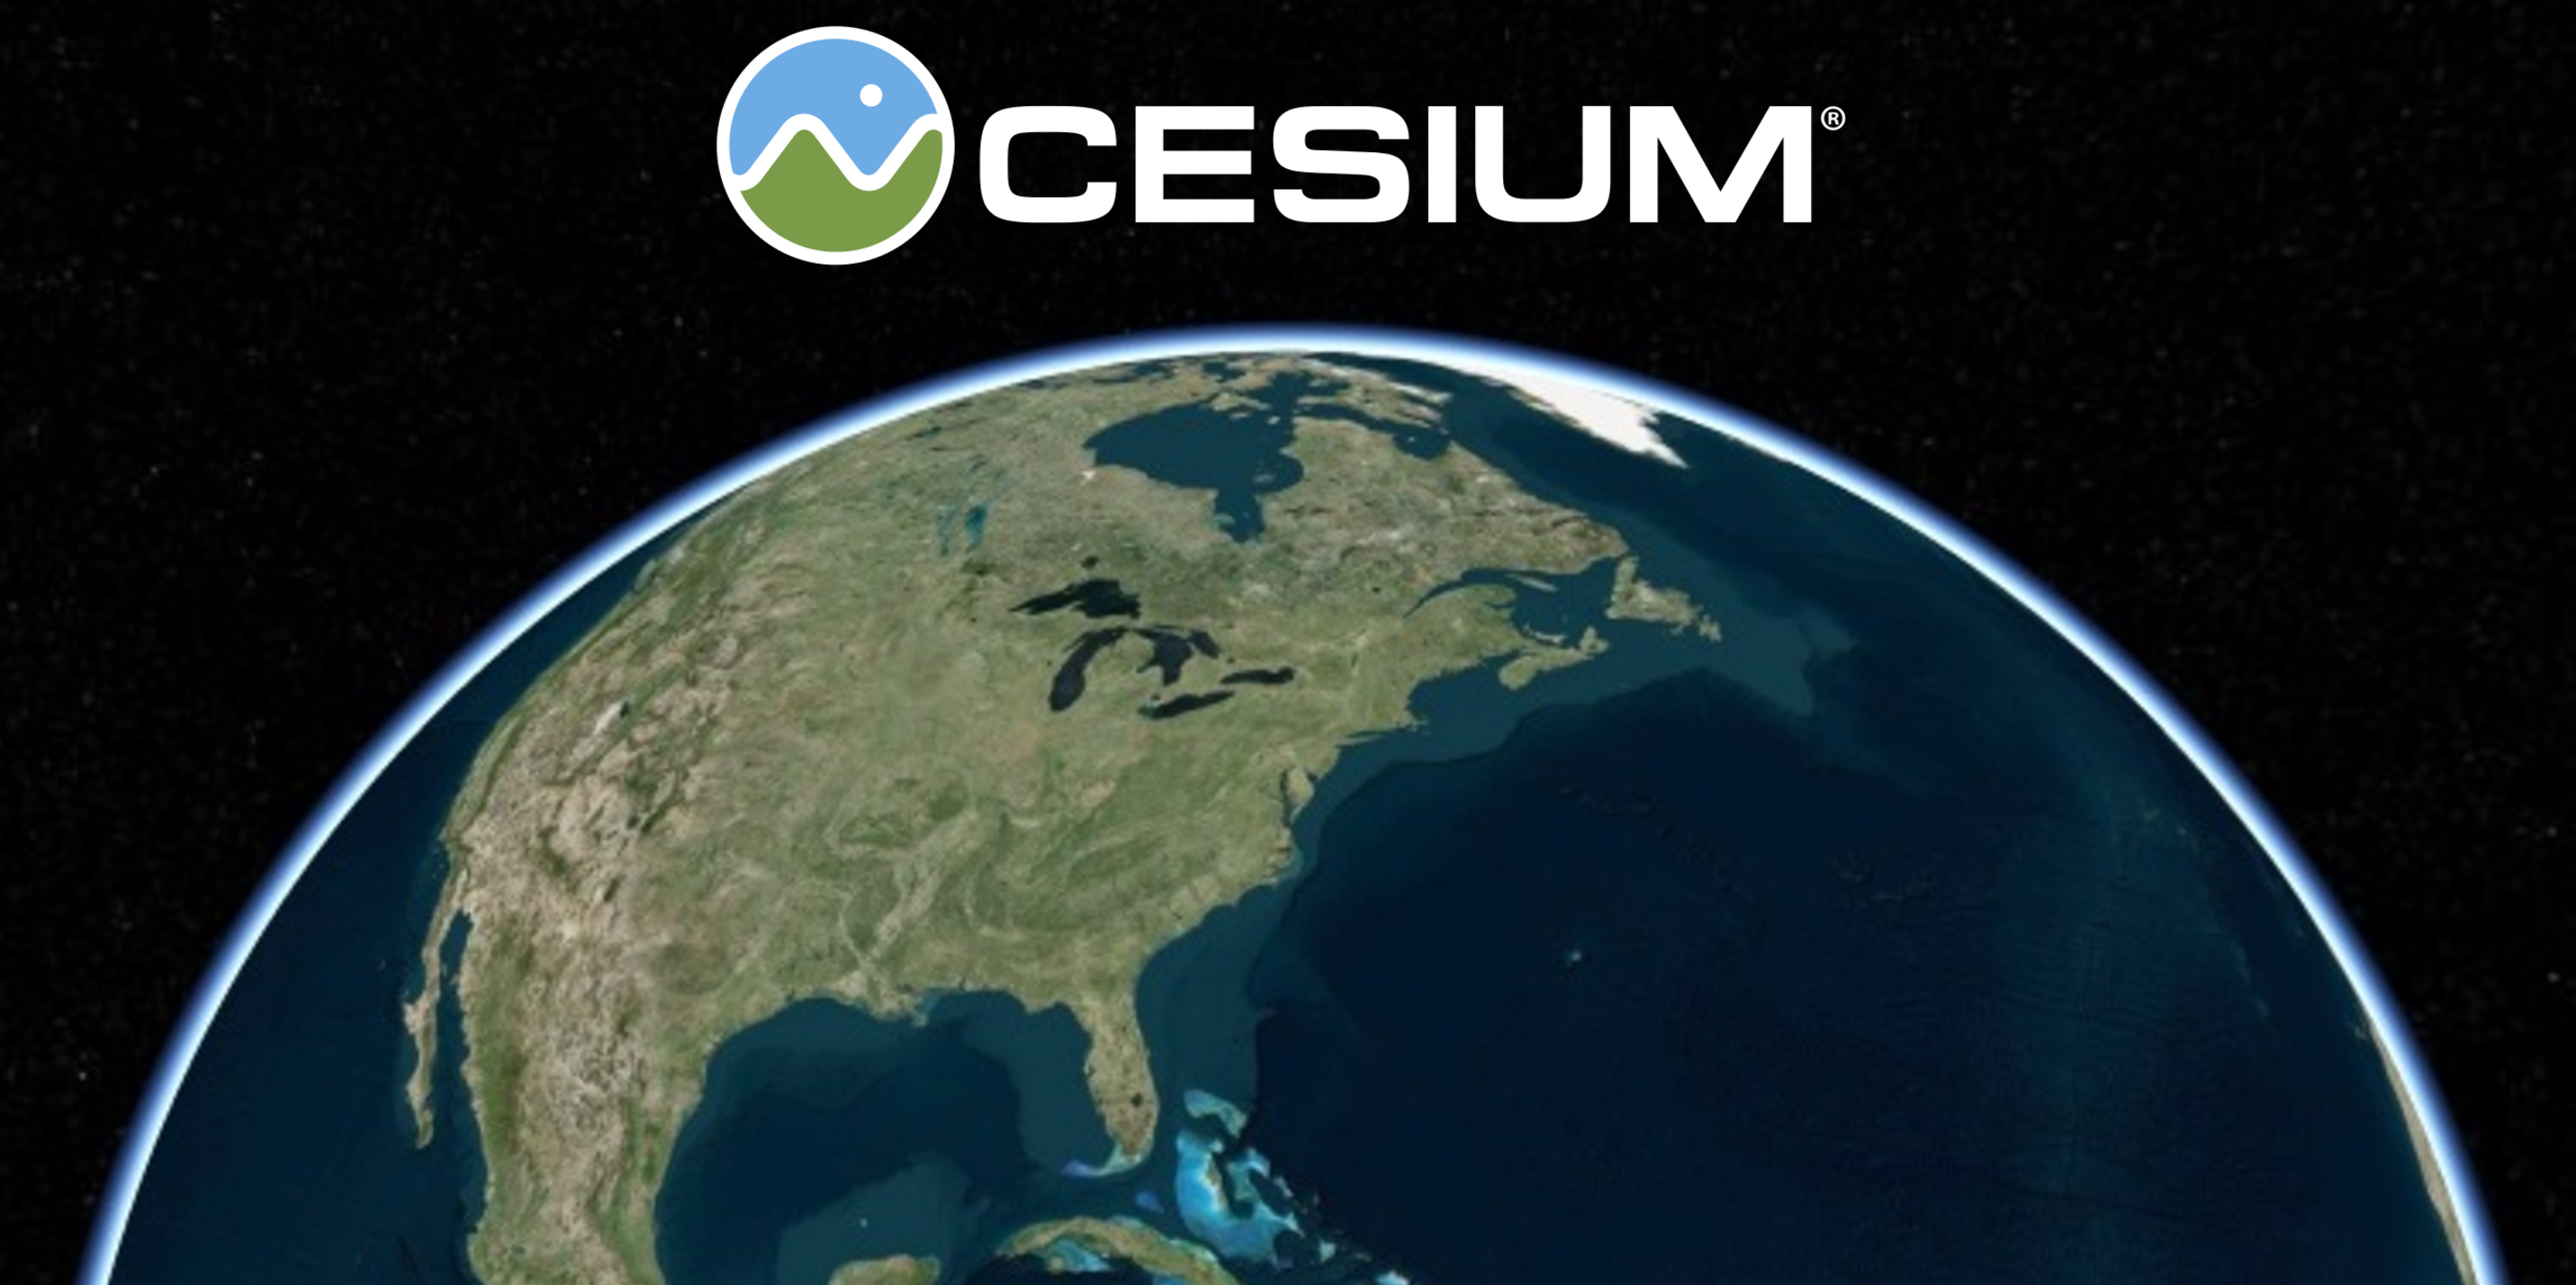
\includegraphics[width=0.4\textwidth]{chapter2/images/cesium_logo}
\caption{Cesium logo}
\label{fig:cesium_logo}
\end{figure}
Cesium\footnote{Cesium: https://cesiumjs.org/} is an open-source JavaScript library for world-class 3D globes and maps that is used to create a web-based globe and map for visualizing dynamic data. This framework runs using WebGL, a JavaScript API for rendering 3D graphics within any compatible web browser that allows GPU--accelerated usage of physics and image processing and effects as part of the web page canvas.\\ 
The features that Cesium provides are the following:
\begin{itemize}
	\item {\bf A virtual globe:} a three-dimensional software model or representation of the Earth that provides the user with the ability to freely move around in the virtual environment by changing the viewing angle and position.
	\item {\bf Different imagery providers:} it allows to draw and layer on high-resolution imagery (maps) from several standard services directly on the virtual globe. 
	\begin{figure} [h]
		\centering
		\begin{subfigure}[b]{0.3\textwidth}
			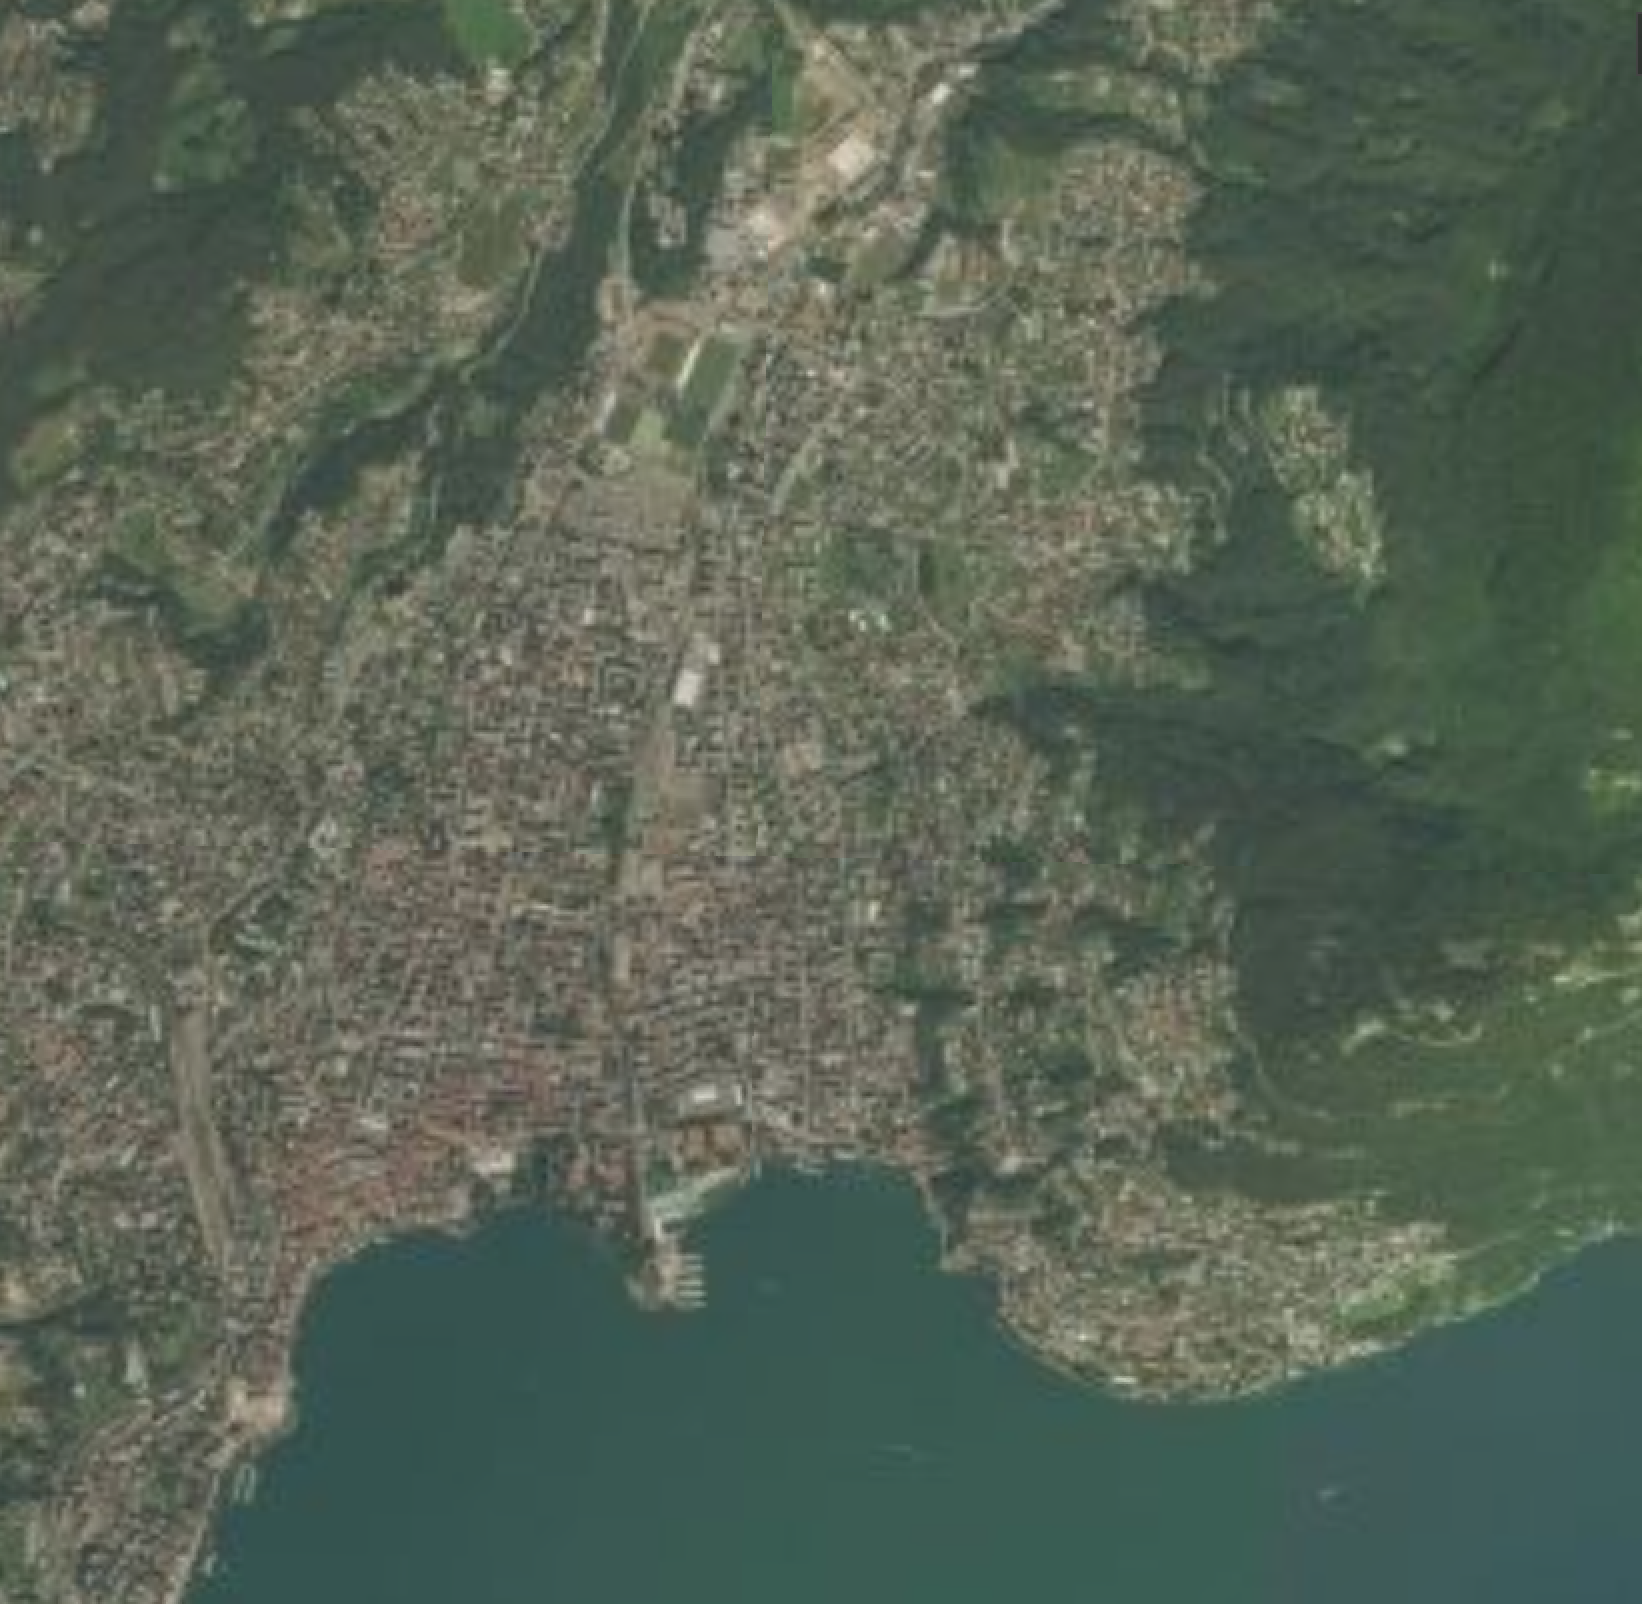
\includegraphics[width=1\textwidth]{chapter2/images/Bing-Map}
			\caption{High-resolution, mesh-based terrain provided by Bing}
			\label{fig:Bing-Map}
		\end{subfigure}
		 \qquad
		\begin{subfigure}[b]{0.3\textwidth}
			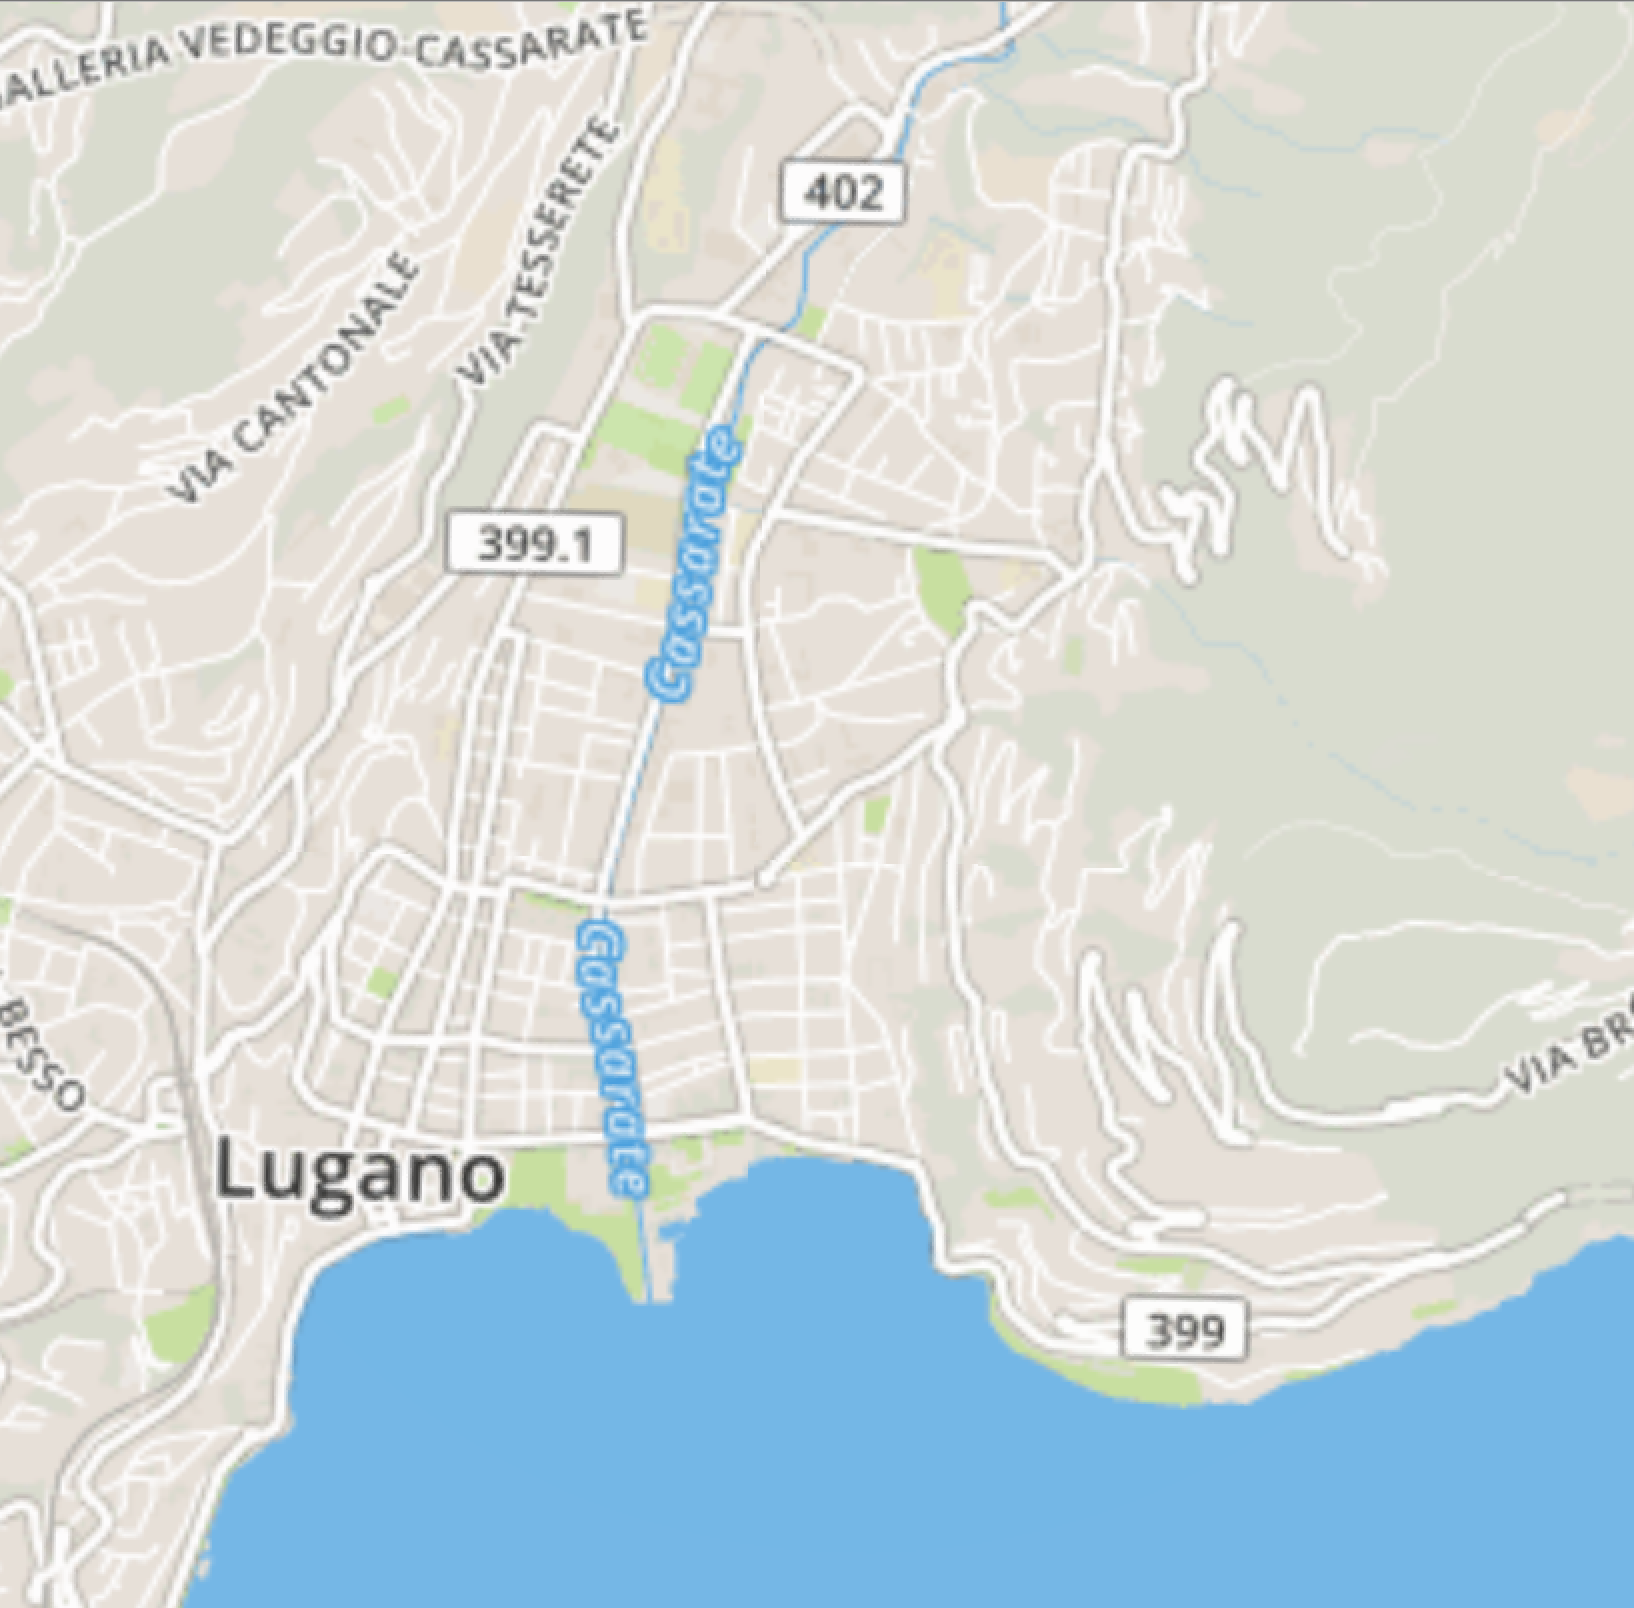
\includegraphics[width=0.993\textwidth]{chapter2/images/Mapbox-Map}
			\caption{Streets basic imagery provided by Mapbox}
			\label{fig:Mapbox-Map}
		\end{subfigure}
		\caption{Example of two imagery providers available on Cesium}
	\end{figure}

	\item {\bf Different terrain providers:} it allows to visualize global high-resolution terrains and water effects for oceans, lakes, and rivers, but mainly the possibility to represent mountain peaks, valleys, and other terrain features. 
	\begin{figure} [H]
		\centering
		\begin{subfigure}[b]{0.3\textwidth}
			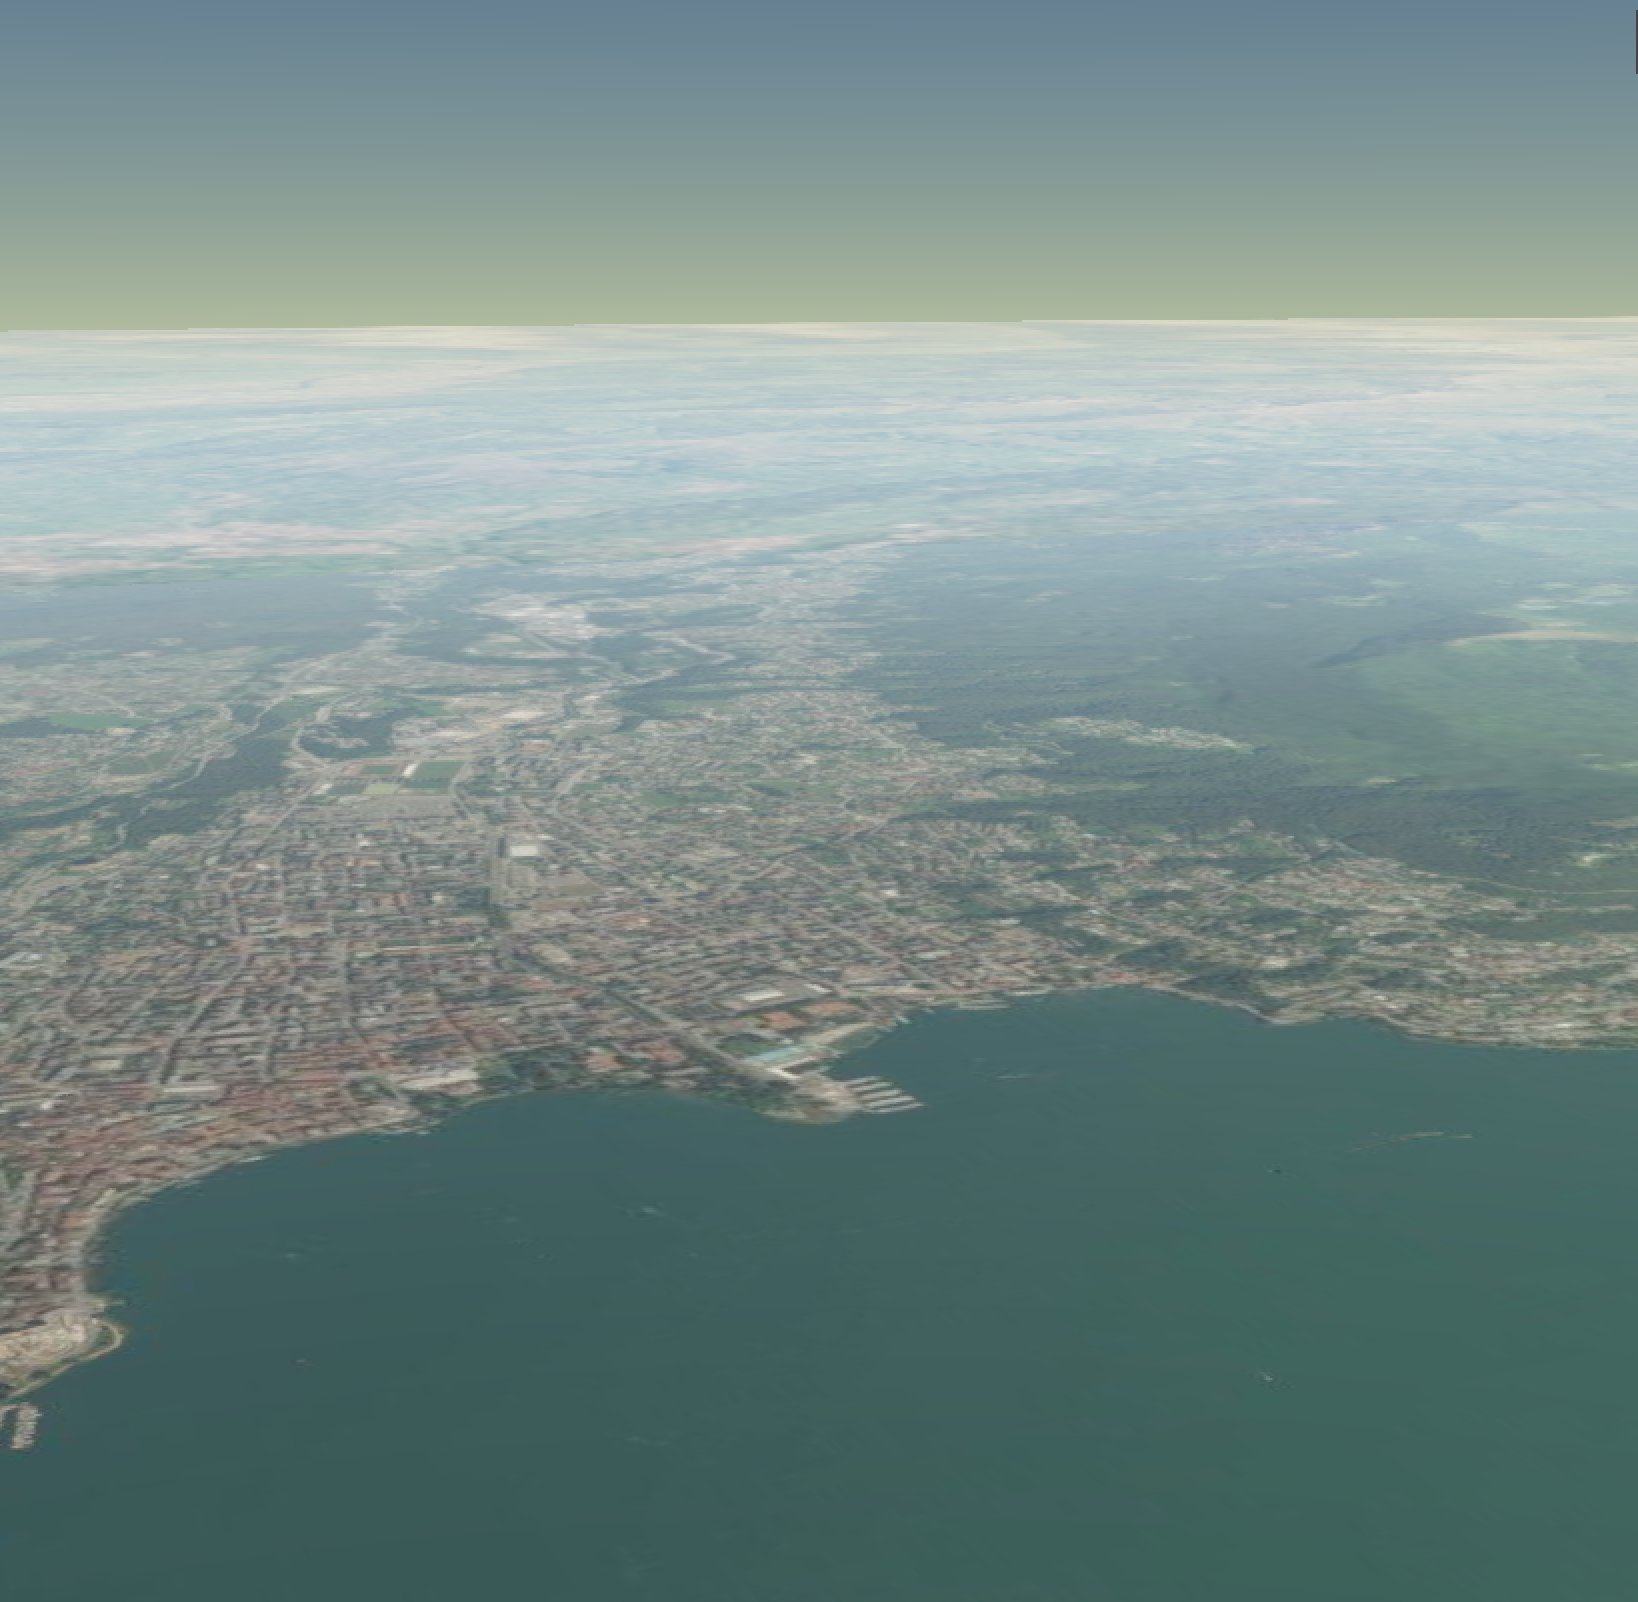
\includegraphics[width=1\textwidth]{chapter2/images/2D-Map}
			\caption{The standard WGS84 Ellipsoid}
			\label{fig:2D-Map}
		\end{subfigure}
		 \qquad
		\begin{subfigure}[b]{0.3\textwidth}
			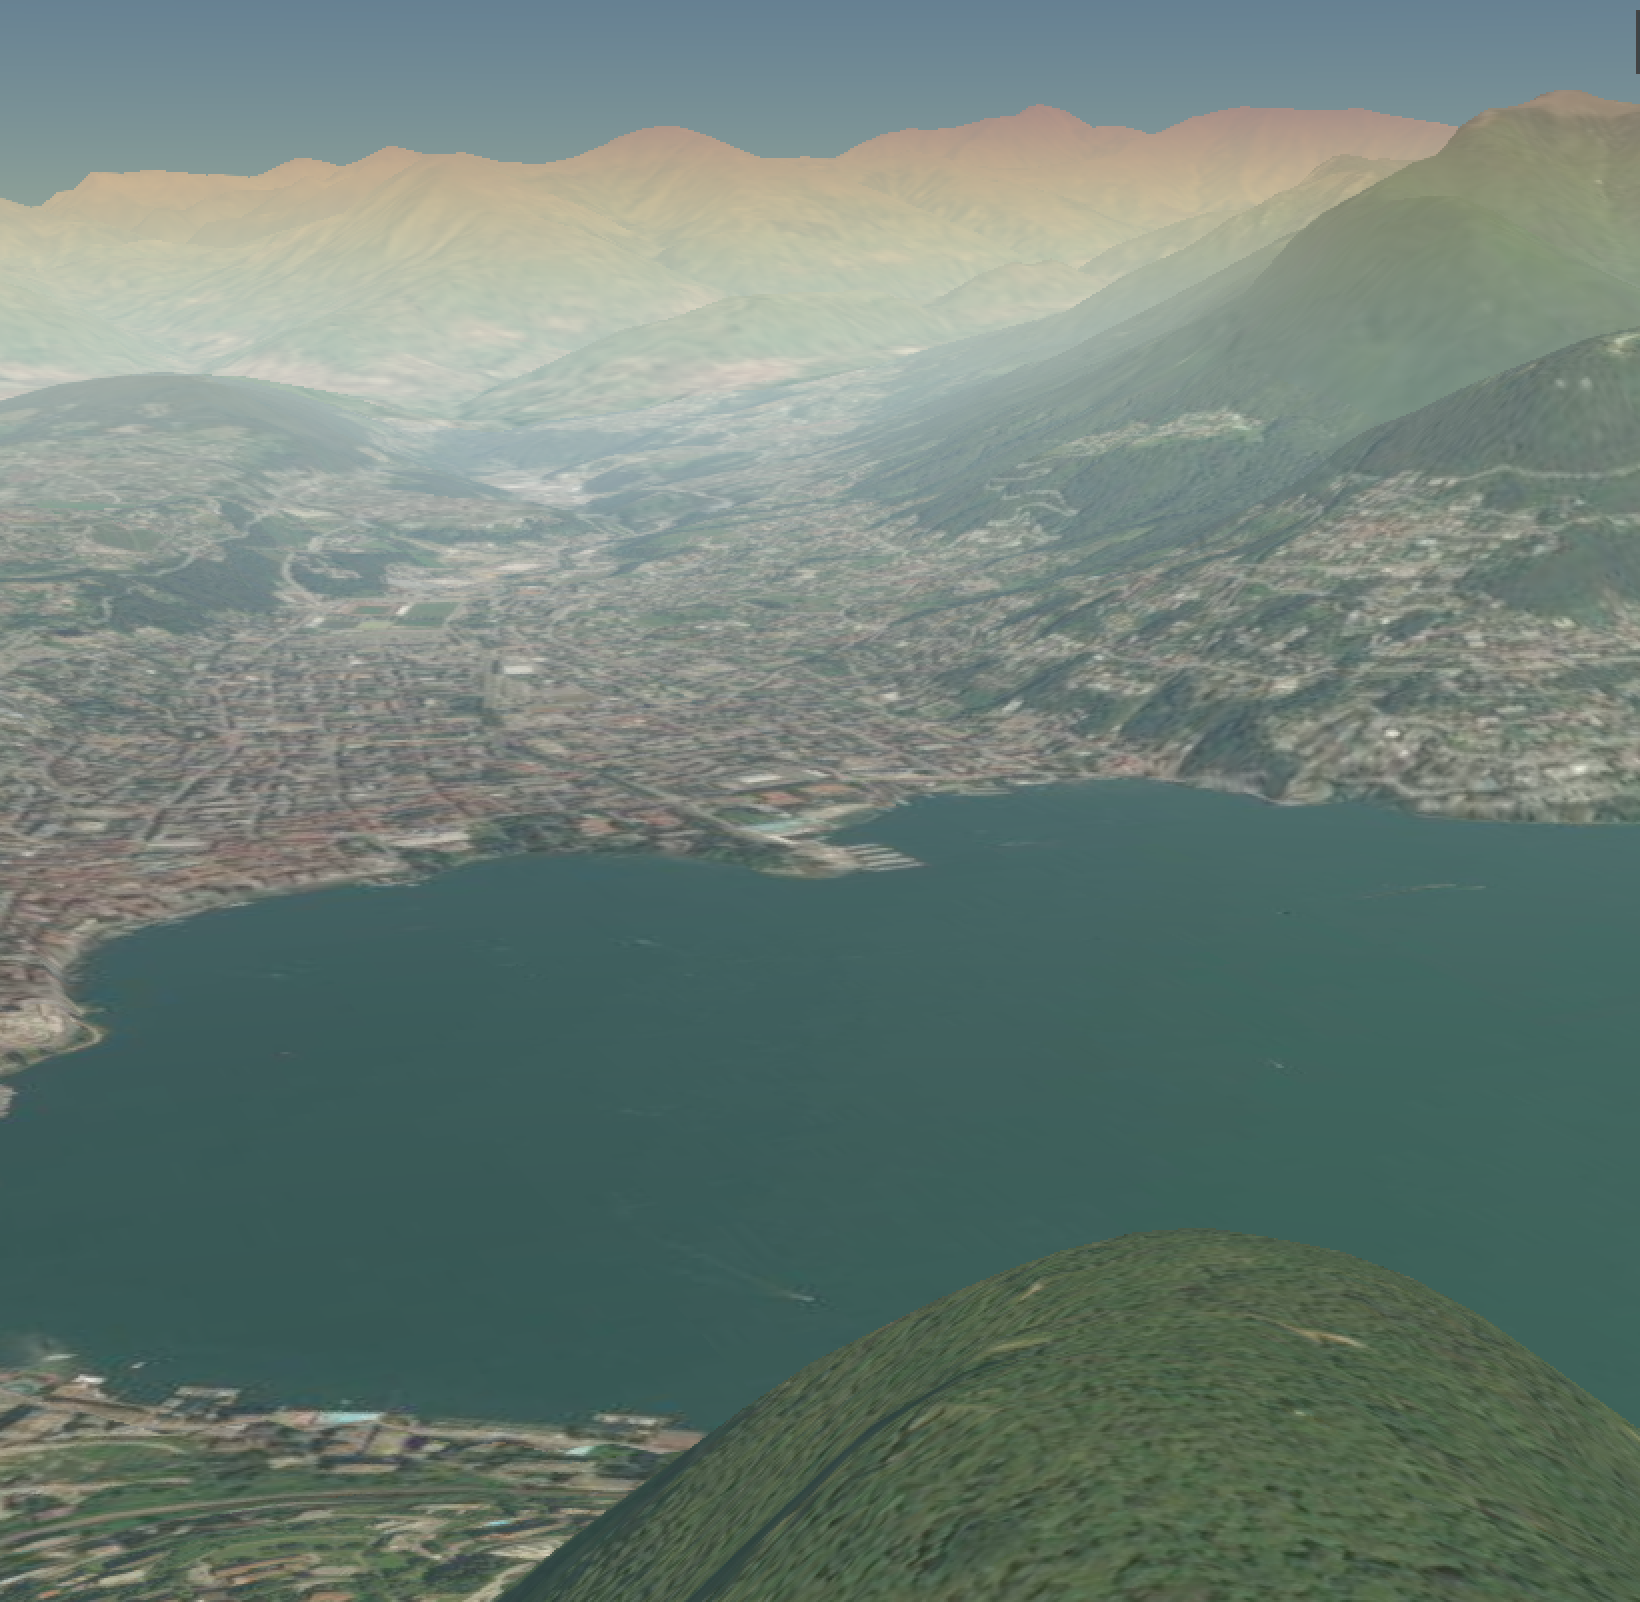
\includegraphics[width=0.993\textwidth]{chapter2/images/3D-Map}
			\caption{Terrain meshes provided by STK}
			\label{fig:3D-Map}
		\end{subfigure}
		\caption{Example of two terrain providers available on Cesium, this shows the benefits of a 3D globe compared to a 2D map.}
	\end{figure}
	\item {\bf Huge number of APIs provided:} since the uses of Cesium are really various, Cesium provides a very high number of APIs in order to control every aspect of the web application, i.e., draw every kind of geometry, handle animations, etc\dots\\The official website of Cesium also provides a complete documentation, various examples, and playgrounds.
\end{itemize}
\begin{center}
	\cfbox{red}{SECTION WORK IN PROGRESS (talk about Cesium 3D Tiles)}
\end{center}
\begin{figure} [H]
\centering
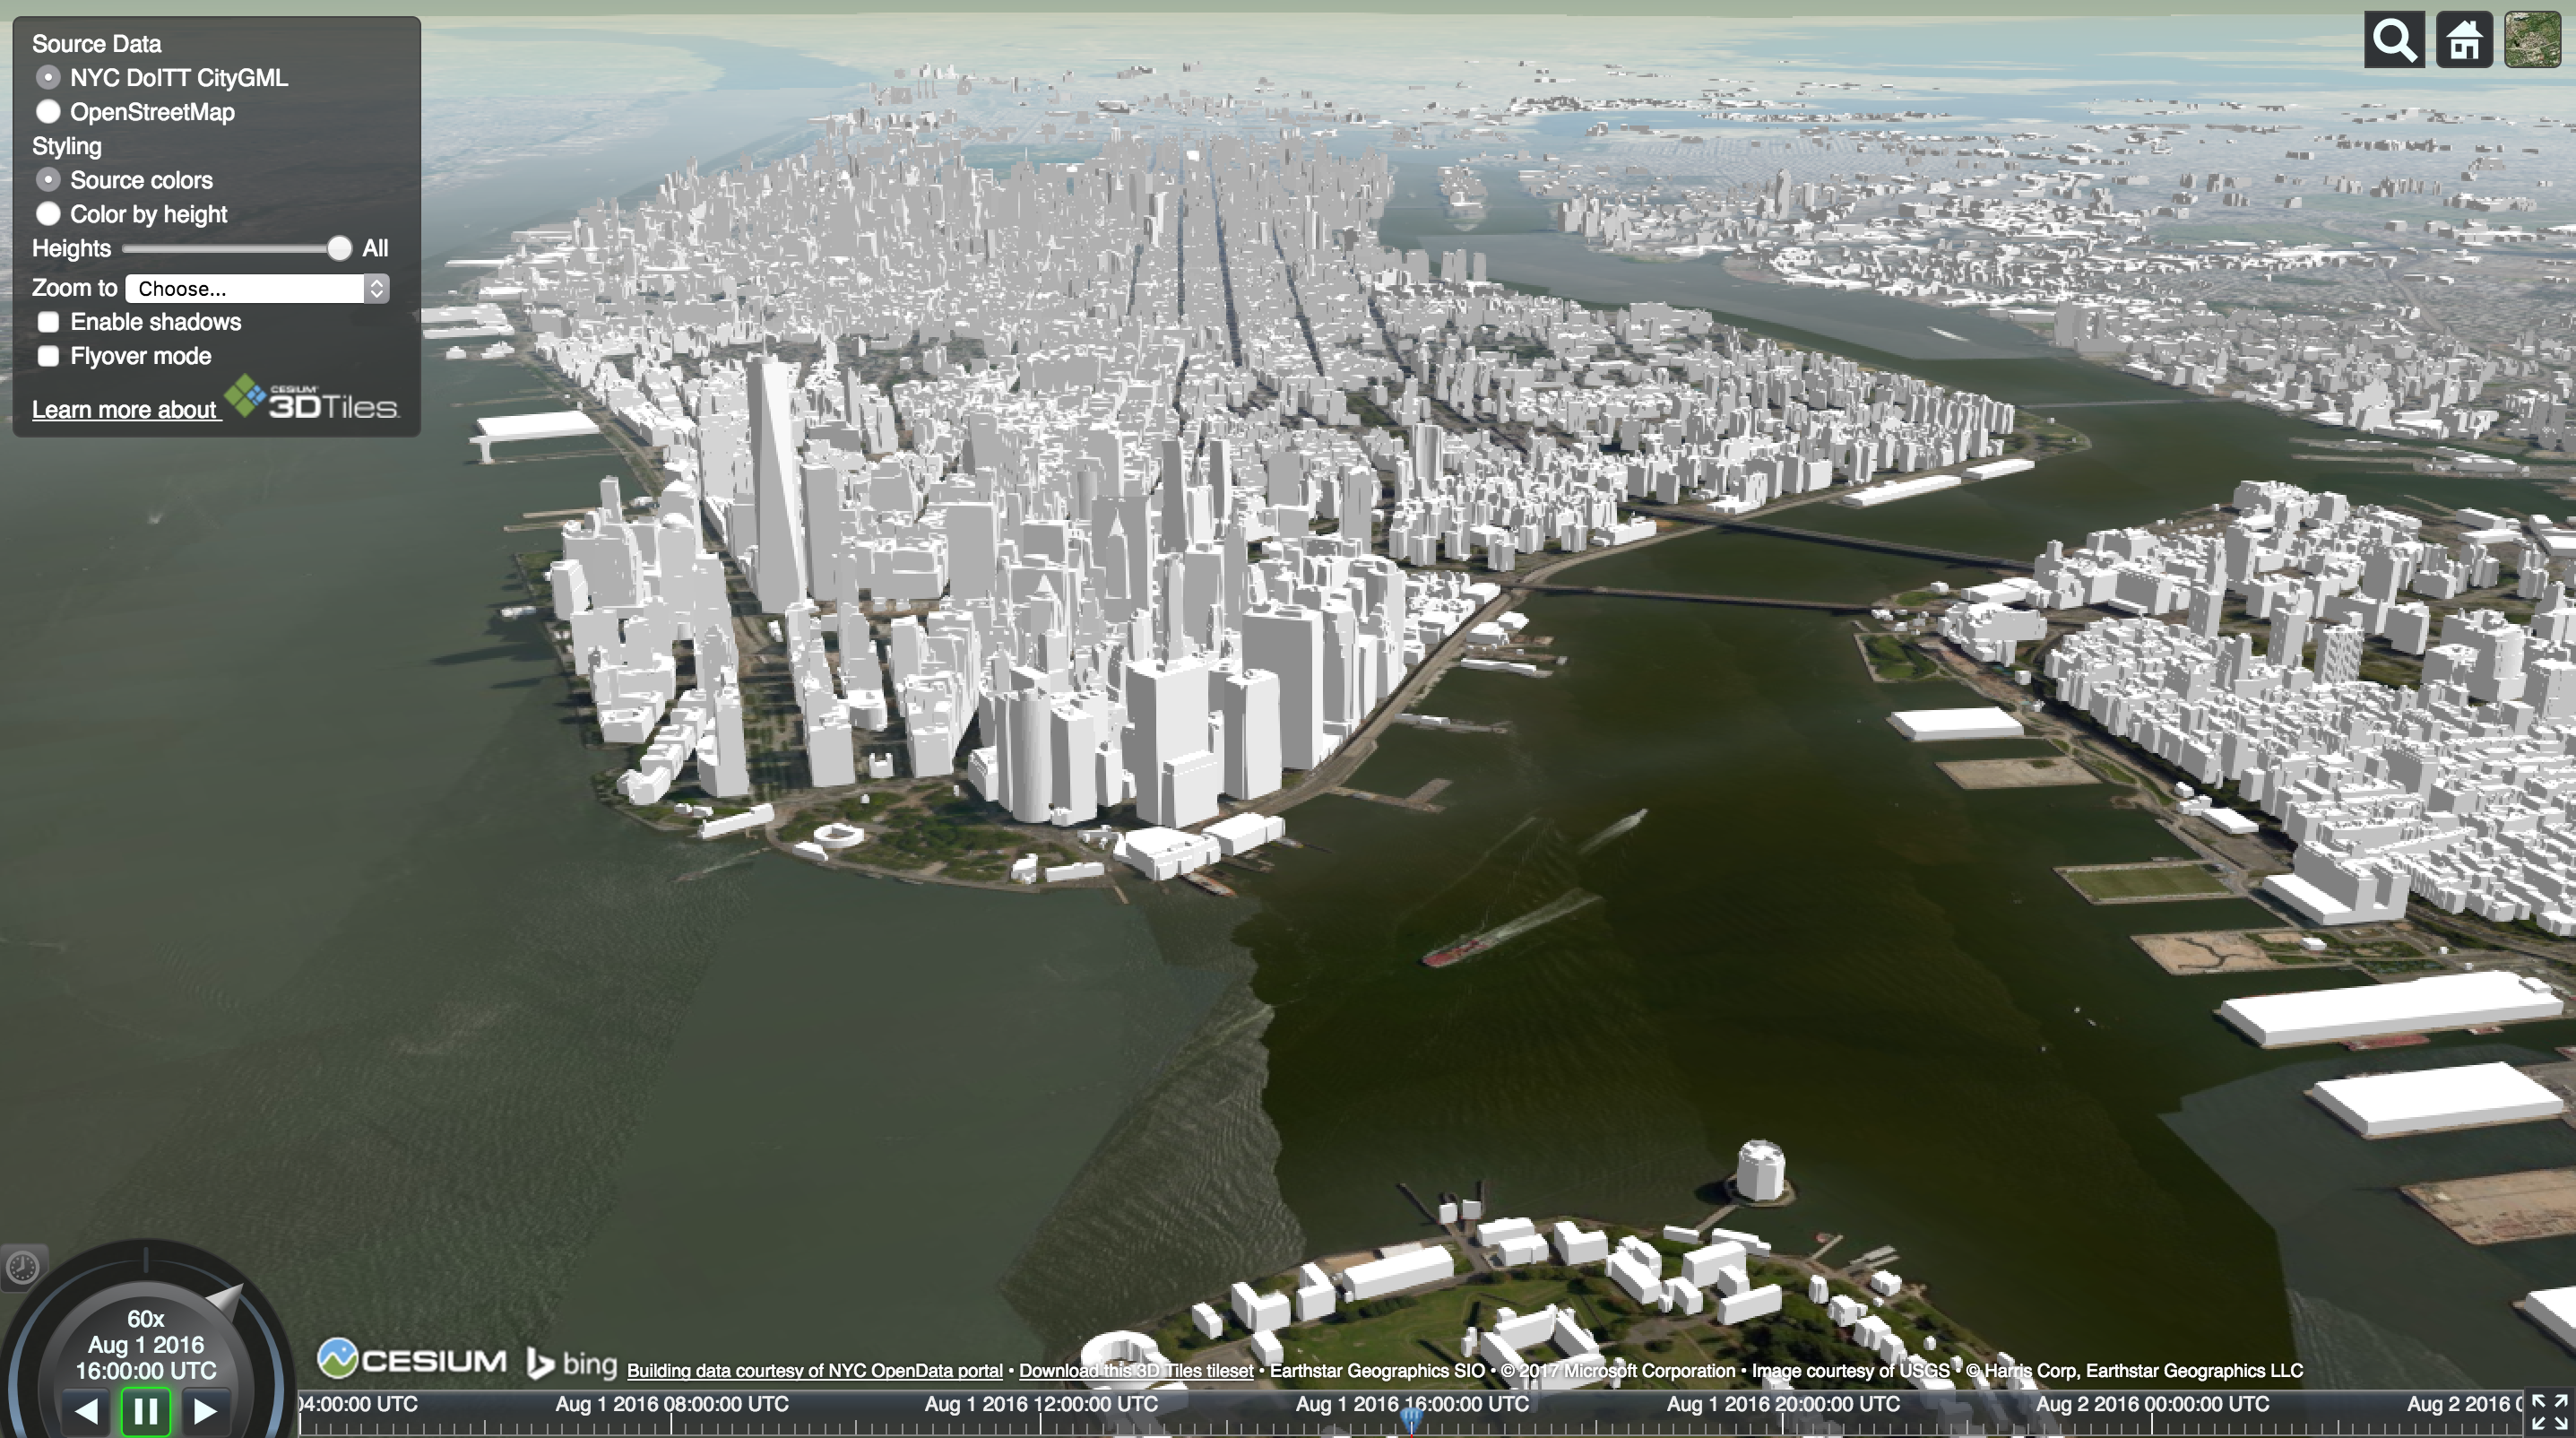
\includegraphics[width=0.8\textwidth]{chapter2/images/NewYorkCityCesium3dTiles}
\caption{An example showing a 3D visualization of the city of New York. Using Cesium 3D Tiles Tecnhology}
\label{fig:NewYorkCityCesium3dTiles}
\end{figure}
\subsection{Swiss Geospatial Portal Using 3D Tiles}
\begin{center}
	\cfbox{red}{SECTION WORK IN PROGRESS}
\end{center}


\begin{figure} [H]
\centering
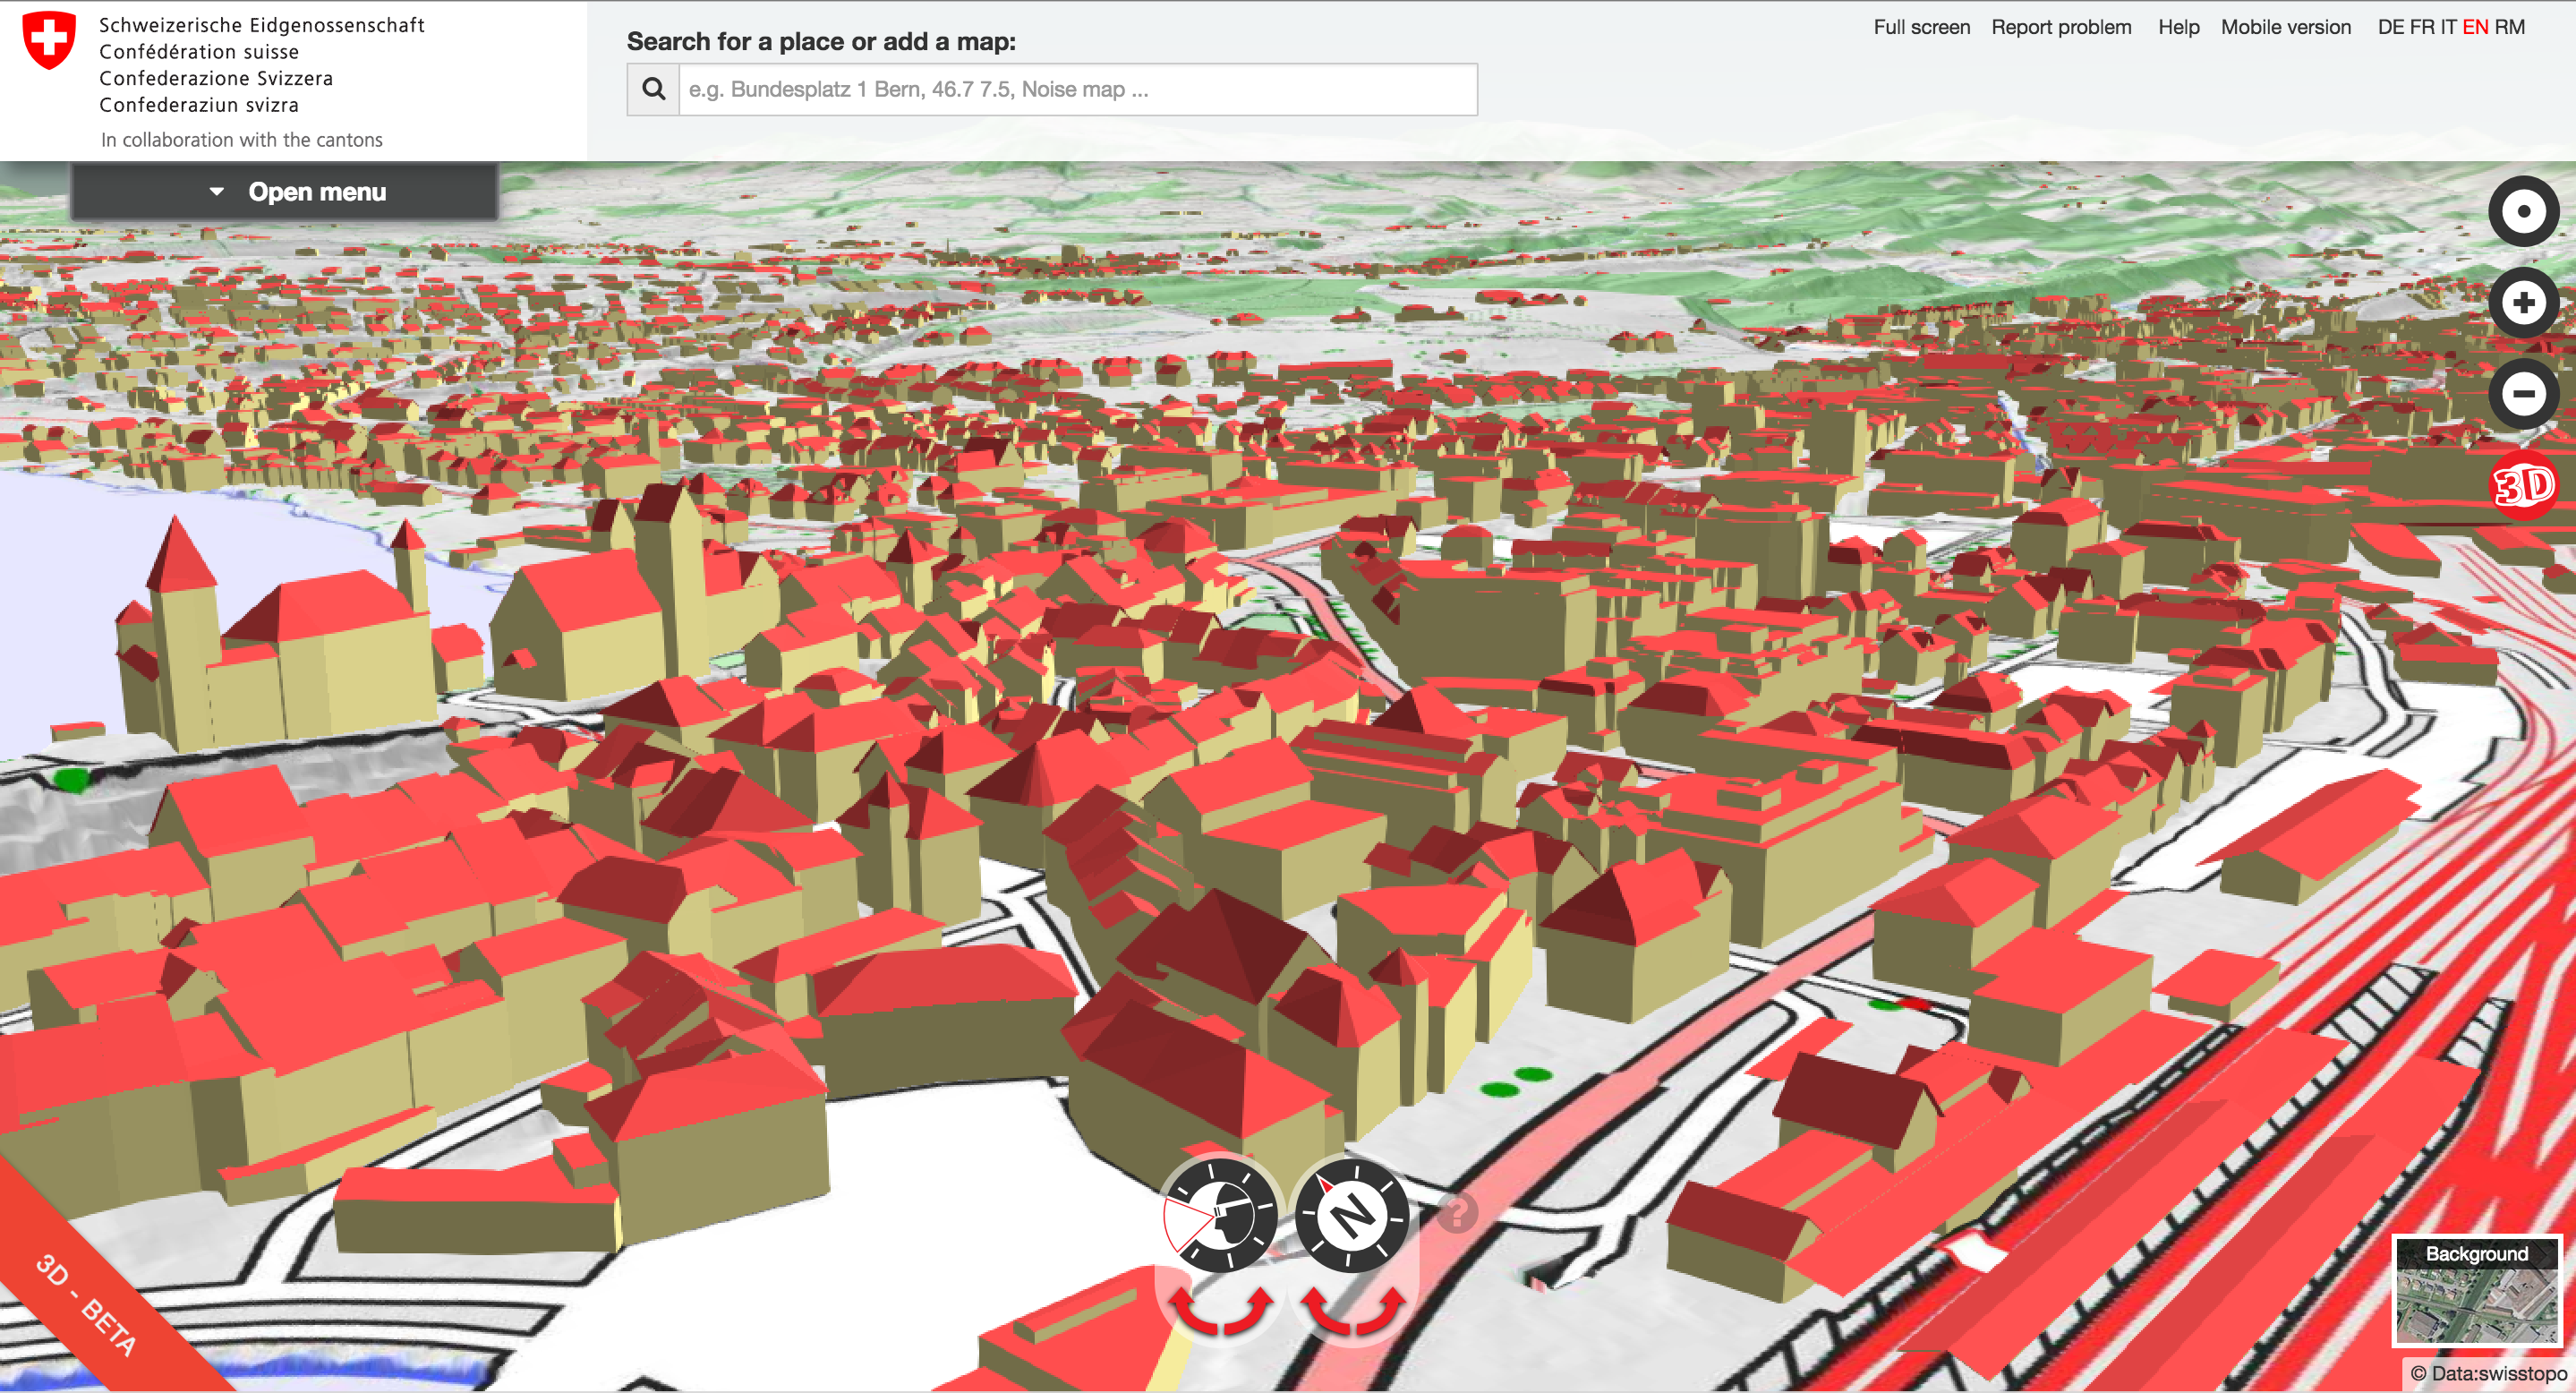
\includegraphics[width=0.8\textwidth]{chapter2/images/BernCitySwissTopo}
\caption{A 3D visualization of the city of Bern in the Swiss Geospatial Portal. Using Cesium 3D Tiles Tecnhology}
\label{fig:BernCitySwissTopo}
\end{figure}